Fine-tuning diffusion language models (DLLMs) extends their flexibility and task adaptability, drawing inspiration from autoregressive (AR) LLM fine-tuning techniques. Recent work demonstrates several viable pathways.

In David helps goliath, the authors report one of the first instances of DLLM fine-tuning by leveraging the DOLLY dataset (15K human-collected instructions and responses) to adapt their SSD-2 diffusion model for downstream tasks. The authors show the finetuned model is better at collaboration than autoregressive counterpart thanks to the bidirectional context reference during ensemble \cite{han_david_2024}.

The \textbf{Mercury Diffusion Language Model} technical report explores alignment-focused fine-tuning strategies: reinforcement learning from human feedback (RLHF) and direct preference optimization (DPO) have been used to guide the diffusion denoiser towards preferred outputs.  By integrating these feedback signals at inference-time trajectories, the model rapidly aligns to user-specified functions, suggesting that DLLMs can match or exceed AR alignment speed \cite{labs2025mercuryultrafastlanguagemodels}.

Supervised fine-tuning (SFT) also proves effective. In Large Language Diffusion Models (LLaDA), the authors demonstrate conventional instruction-driven SFT on a diffusion backbone, showing scalable improvements in generative accuracy across a range of tasks.  By framing instructions as conditioning masks in the denoising process, DLLMs achieve comparable zero-shot performance to AR LLMs post-finetuning \cite{nie_large_2025}.

Beyond standard SFT, Instruction Fine-Tuning further enhances generalization.  \textbf{Diffusion Language Models Can Perform Many Tasks with Scaling and Instruction-Finetuning} shows instruction-tuned diffusion models generalize to unseen languages and tasks without additional data. E.g., German text generation emerges zero-shot after English only fine-tuning and highlighting the strong transfer capacity of DLLMs \cite{ye_diffusion_2025}.

These studies reveal a promising interpolation between AR and diffusion fine-tuning. Parameter-efficient adapters and instruction masks can be seamlessly adapted to the denoising architecture; this enables rapid specialization and alignment.  Potential future work includes integrating LoRA - low-rank adaptation techniques to reduce tuning overhead and explore hybrid schedules that jointly adjust AR and diffusion components during fine-tuning.

\begin{figure*}[ht]
    \centering
    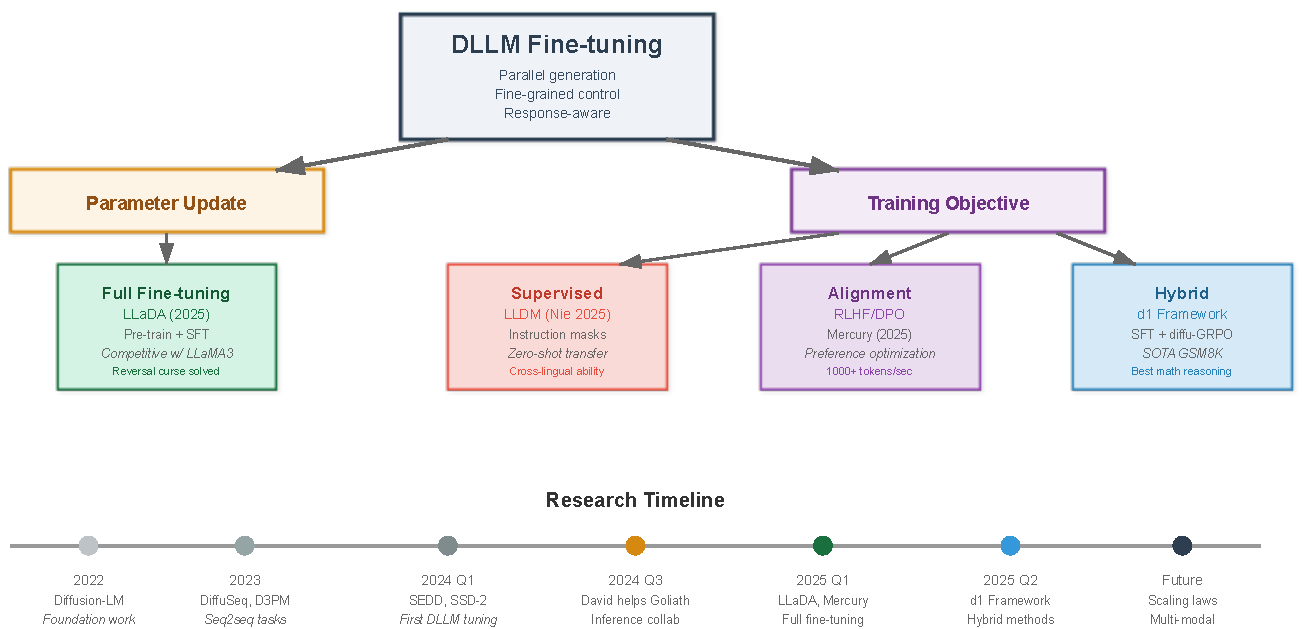
\includegraphics[width=0.9\textwidth]{figs/10_finetune.pdf}
    \caption{DLLM Fine-tuning Methods: Taxonomy and Evolution}
    \label{fig:dllm_finetune}
\end{figure*}

% \bibliographystyle{plain}
% \bibliography{DLLM}